\documentclass[12pt]{report}

\usepackage[utf8]{inputenc}
\usepackage[T1]{fontenc}
\usepackage{mathpazo}
\usepackage{multirow}
\usepackage{hyperref}
\usepackage{caption,subcaption}
\usepackage{multirow}
\usepackage{amsmath}
\usepackage{placeins}

\usepackage[margin=1in]{geometry}

\usepackage{graphicx}
\graphicspath{{./images}}


\title{Applying tabu search to the capacitated vehicle routing problem}
\author{Phan Ngoc Lan}

\begin{document}

\begin{titlepage}
	\newcommand{\HRule}{\rule{\linewidth}{0.5mm}} % Defines a new command for horizontal lines, change thickness here

	\center % Centre everything on the page

	%------------------------------------------------
	%	Headings
	%------------------------------------------------

	\textsc{\large Hanoi University of Science and Technology}\\[1.5cm] % Main heading such as the name of your university/college

	\textsc{\large Seminar 1: Metaheuristics}\\[0.5cm] % Major heading such as course name

	\textsc{\large IT5422E}\\[0.5cm] % Minor heading such as course title

    %------------------------------------------------
	%	Logo
	%------------------------------------------------

	% \vfill\vfill
	
\includegraphics[height=100px]{hust.png}\\[1cm] % Include a department/university logo - this will require the graphicx package

	%------------------------------------------------
	%	Title
	%------------------------------------------------

	\HRule\\[0.4cm]

	{\huge\bfseries Applying tabu search to the capacitated vehicle routing problem}\\[0.4cm] % Title of your document

	\HRule\\[1.5cm]

	%------------------------------------------------
	%	Author(s)
	%------------------------------------------------

	\begin{minipage}{0.4\textwidth}
		\begin{flushleft}
			\large
			\textit{Author}\\
			\textsc{Phan} Ngoc Lan % Your name
		\end{flushleft}
	\end{minipage}
	~
	\begin{minipage}{0.4\textwidth}
		\begin{flushright}
			\large
			\textit{Supervisor}\\
			Dr. Michel \textsc{Toulouse} % Supervisor's name
		\end{flushright}
	\end{minipage}

	% If you don't want a supervisor, uncomment the two lines below and comment the code above
	%{\large\textit{Author}}\\
	%John \textsc{Smith} % Your name

	%------------------------------------------------
	%	Date
	%------------------------------------------------

	\vfill\vfill\vfill % Position the date 3/4 down the remaining page

	{\large\today} % Date, change the \today to a set date if you want to be precise

	\vfill % Push the date up 1/4 of the remaining page
\end{titlepage}

\tableofcontents
\pagebreak

\chapter{Introduction}
\section{The capacitated vehicle routing problem}
Vehicle routing problems (VRPs) are some of the most well-studied and widely-applied optimization problems. The first definitions of VRP were presented by Dantzig et al. \cite{dantzig1959truck} in 1959. In general, VRPs seek to find an optimal set of tours for a fleet of vehicles to service a set of customers. Optimality may refer to minimizing costs, or maximizing overall profits. This abstraction covers a wide variety of application domains, including transportation, logistics, operations, etc \dots

Since its conception, a number of variants of the VRP have been proposed through the years. These variants account for different constraints as well as optimization goals. Popular VRP variants include:
\begin{itemize}
	\item Capacitated Vehicle Routing Problem (CVRP): vehicles have capacity constraints;
	\item Vehicle Routing Problem with Time Windows (VRPTW): customers have time windows outside of which they cannot be serviced;
	\item Vehicle Routing Problem with Profits (VRPP): customers have profit values, and may not be serviced;
	\item etc \dots
\end{itemize}

This report focuses on solving the capacitated vehicle routing problem. CVRP is one of the most basic VRP variants. The problem considers a set of $n$ customers, each with a demand value $d_i$. Conversely, each vehicle has a capacity $C$, which is uniform among all vehicles. The CVRP states that no route can have a total demand (the sum of all customers' demands) exceeding the capacity $C$. Vehicle routes always start and end at a pre-determined location, called the depot. We seek a set of $k \leq n$ valid routes such that all customers are serviced \textit{exactly} once, and the total cost is minimized. Commonly, the depot and customer locations are set on a 2D space, where moving from location $A$ to location $B$ incurs a cost equal to the Euclidean distance between $A$ and $B$. Figure \ref{fig:prob_example} shows an example of CVRP input and solution.

\begin{figure}[]
    \centering
    \begin{subfigure}[b]{0.49\linewidth}
        \centering
        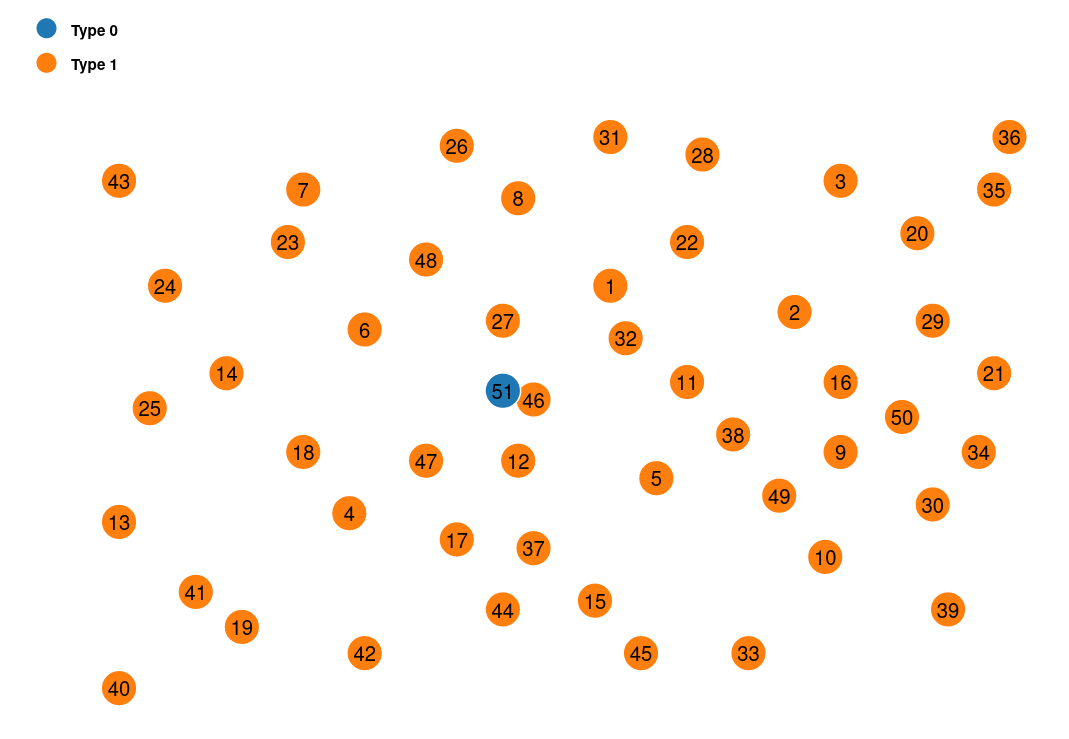
\includegraphics[width=0.95\textwidth]{images/cmt01.png}
        \caption{Problem input}
    \end{subfigure}
    \begin{subfigure}[b]{0.49\linewidth}
        \centering
        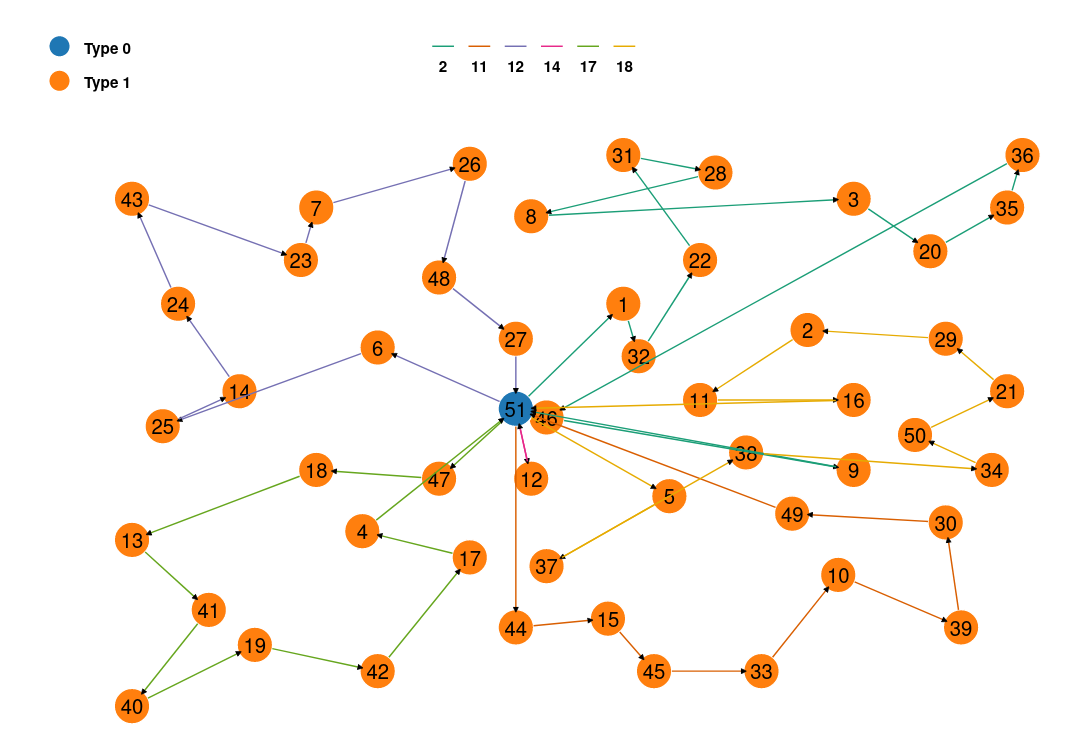
\includegraphics[width=0.95\textwidth]{images/cmt01_solution.png}
        \caption{Example output}
    \end{subfigure}
    \caption{Input and example output for CVRP instance CMT01 in the Christofides CMT dataset. The blue node denotes the depot, orange nodes denote customer locations. Visualization made using VRP-REP Mapper \protect\footnotemark }
	\label{fig:prob_example}
\end{figure}

\footnotetext{https://vrp-rep.github.io/mapper/}

\section{Formulation}
Formally, the CVRP is defined as (\cite{borcinova2017two}):

\begin{equation}
    min \sum_{r=1}^p \sum_{i=0}^n \sum_{j=0, i \neq j}^n c_{ij}x_{rij} \label{eq:form1}
\end{equation}
subject to
\begin{align}
    \sum_{r=1}^p \sum_{i=0,i \neq j}^n x_{rij} = 1 \ & \forall j \in \{1, \dots, n\} \label{eq:form2} \\
    \sum_{j=1}^n x_{r0j} = 1 \ & \forall r \in \{1,\dots,p\} \label{eq:form3} \\
    \sum_{i=0,i \neq j} x_{rij} = \sum_{i=0} x_{rji} \ & \forall j \in \{1, \dots, n\},\ r \in \{1,\dots,p\} \label{eq:form4} \\
    \sum_{i=0}^n \sum_{j=1,i \neq j} d_j x_{rij} \leq Q \ & \forall r \in \{1,\dots,p\} \label{eq:form5} \\
    \sum_{r=1}^p \sum_{i \in S} \sum_{j \in S, i \neq j} x_{rij} \geq |S| - 1 \ & \forall S \subseteq \{1,\dots,n\} \label{eq:form6} \\
    x_{rij} \in \{ 0, 1 \} \ & \forall i,j \in \{0, \dots, n\},\ r \in \{1,\dots,p\} \label{eq:form7}
\end{align}
where
\begin{itemize}
	\item $V = \{0, 1, \dots, n\}$ is the set of locations. $0$ is the depot, where vehicles must start and end their routes;
	\item $p$ is the maximum number of vehicles. If not specified, we can let $p = n$;
	\item $c_{ij}$ is the cost of including edge $(i, j)$ in a route, or the cost incurred when moving from from $i$ to $j$;
	\item $x_{rij}$ is the binary variable signifying whether the edge $(i,j)$ is included in route $r$;
	\item $d_j$ denotes the demand for location $j$;
	\item $Q$ is the vehicle capacity.
\end{itemize}

\section{The Clarke-Wright algorithm}
The Clarke-Wright algorithm, sometimes referred to as the savings algorithm, is a very simple method for generating a valid solution to the CVRP. This is a greedy heuristic that is not optimal, but is often used as the basis for many metaheuristic algorithms.

The Clarke-Wright algorithm defines a savings value for each edge $(i,j)$:
\[
	s_{ij} = c_{i0} + c_{0j} - c_{ij}
\]

An edge's savings value denotes the amount of "cost" that can be saved by replacing two routes, $(0, i, 0)$ and $(0, j, 0)$ with a new route $(0, i, j, 0)$.

The algorithm first calculates the savings for each non-depot edge, then sorts them in a descending order, forming the savings list. $n$ routes are created, each starting at the depot, visits one customer, then returns. Then, the savings list is iterated one-by-one. For each edge $(i, j)$, check for 3 conditions:
\begin{enumerate}
	\item $i$ and $j$ must not be on the same route;
	\item $i$ and $j$ must still be connected to the depot on each of their routes;
	\item Merging the routes containing $i$ and $j$ will not violate the capacity constraints.
\end{enumerate}

If all 3 conditions are met, the routes containing $i$ and $j$ are merged, by appending $j$ after $i$ and then returning to the depot.

Each route join in the Clarke-Wright algorithm is guaranteed to improve the solution by the amount of edge savings. However, the greedy ordering is non-optimal, meaning we are likely to skip edges that would otherwise be part of the optimal solution.

\chapter{Tabu search and CVRP}
\section{Tabu search}

\section{SimpleTabu}
This section describes SimpleTabu, a tabu search for solving the CVRP. SimpleTabu is a full tabu search with 3 phases: short-term, intensification, and diversification.

\begin{itemize}
	\item The short-term phase performs a search using only the tabu list, excluding previous moves from the search to avoid local minima;
	\item The intensification phase selects a promising area in the search and explores it further, becoming more lenient with local minima;
	\item The diversification phase tries to move the search to a new, unexplored area, in order to find more promising solutions.
\end{itemize}

The search procedure starts with an initial solution. The short-term phase is run first, in which long-term memory objects are updated. Upon termination, a new initial solution is selected to start the intensification phase. After this phase, another initial solution is created for diversification.

\subsection{Initialization}
SimpleTabu uses the Clarke-Wright algorithm to create its initial solution. However, the original Clarke-Wright algorithm is deterministic, which can hinder a search. A simple way to introduce randomness is adding weights to the savings list. The savings value for each edge can be multiplied with a predetermined weight $w_{ij}$. A randomly generated weight matrix would then allow us to subtly randomize the output without breaking constraints.

\subsection{Neighborhood space}
The neighborhood space for SimpleTabu is constructed from a combination of neighbor operators. A large number of operators have been proposed for the CVRP, for example as seen in \cite{mcnabb2015testing}. In this report, we examine 3 operators:
\begin{enumerate}
	\item Relocate: Move a location on a single route;
	\item 2-opt*: Swap two locations on two different routes;
	\item Or-opt: Attach a random segment from one route to another route.
\end{enumerate}

Figure \ref{fig:operators} further illustrates the above operators.

\begin{figure}[ht]
	\centering
	\begin{subfigure}[b]{\linewidth}
		\centering
		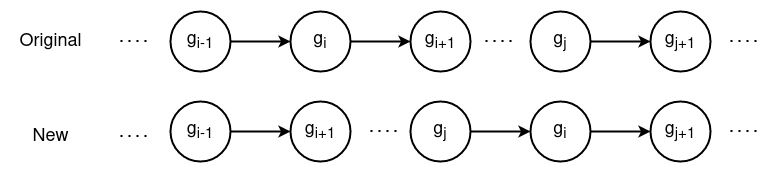
\includegraphics[width=0.7\textwidth]{images/lsops-relocate.png}
		\caption{Relocate}
	\end{subfigure}
	\begin{subfigure}[b]{0.35\linewidth}
		\centering
		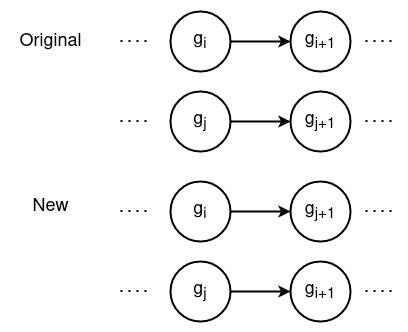
\includegraphics[width=0.95\textwidth]{images/lsops-2-opt.png}
		\caption{2-opt*}
	\end{subfigure}
	\begin{subfigure}[b]{0.63\linewidth}
		\centering
		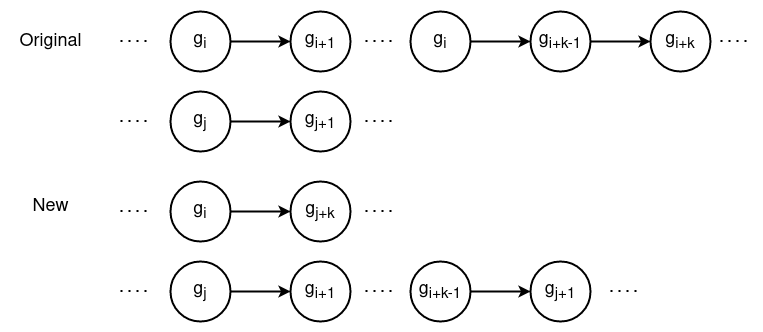
\includegraphics[width=0.95\textwidth]{images/lsops-or-opt.png}
		\caption{Or-opt}
	\end{subfigure}
	\caption{Visualizations of local search operators used by SimpleTabu}
	\label{fig:operators}
\end{figure}

In each search iteration, SimpleTabu generates neighbors using all operators, merges them and samples a fixed-size candidate set from this population.

\subsection{Intensification}

\section{Related works}

\chapter{Experiments and results}
\section{Experiment settings}
We shall examine 2 experiments:
\begin{itemize}
	\item Ablation study: different combinations of neighborhoods are compared, in order to make conclusions on each neighbor's effectiveness;
	\item Comparison: SimpleTabu is compared against two existing methods, ALNS \cite{pisinger2007general} and GRELS \cite{prins2009grasp}.
\end{itemize}

The SimpleTabu algorithm is implemented in Python 3.7, and executed using the PyPy \cite{rigo2006pypy} runtime. All runs are performed on a single 2-core AMD EPYC 2.2Ghz CPU with 4GB RAM.

Experiments are performed using instances from the Christofides et al. dataset \cite{christofides1976vehicle}, which includes 14 CVRP instances of medium size.

Hyperparameters for SimpleTabu are shown in Table \ref{tab:tabu-params}.

\begin{table}[htp]
\centering
\begin{tabular}{|l|r|}
    \hline
    \multicolumn{1}{|c|}{\textbf{Parameter}} & \multicolumn{1}{c|}{\textbf{Value}} \\ \hline
    Short-term max iters. & 300 \\ \hline
    Short-term early-stop tolerance & 10 \\ \hline
    Short-term tabu list size & 300 \\ \hline
    Intensification max iters. & 300 \\ \hline
    Intensification early-stop tolerance & 5 \\ \hline
    Intensification tabu list size & 200 \\ \hline
    Diversification max iters. & 300 \\ \hline
    Diversification early-stop tolerance & 20 \\ \hline
    Diversification tabu list size & 400 \\ \hline
    Candidate set size & 3000 \\ \hline
    Elite set size & 10 \\ \hline
\end{tabular}
\caption{Parameter values for SimpleTabu}
\label{tab:tabu-params}
\end{table}


\section{Results and discussion}
\subsection{Ablation study}

\begin{table}[]
\resizebox{\textwidth}{!}{
\begin{tabular}{ |c|r|r|r|r|r|r|r|r| }
\hline
\multicolumn{1}{|c|}{ \multirow{2}{*}{ \textbf{ Instance } } } & \multicolumn{2}{|c|}{ \textbf{ SimpleTabu (Full) } } & \multicolumn{2}{|c|}{ \textbf{ SimpleTabu (No Or-Opt) } } & \multicolumn{2}{|c|}{ \textbf{ SimpleTabu (No 2-Opt*) } } & \multicolumn{2}{|c|}{ \textbf{ SimpleTabu (No Relocate) } } \\
\cline{ 2-9 }
 & \multicolumn{1}{|c|}{ Best } & \multicolumn{1}{|c|}{ Std } & \multicolumn{1}{|c|}{ Best } & \multicolumn{1}{|c|}{ Std } & \multicolumn{1}{|c|}{ Best } & \multicolumn{1}{|c|}{ Std } & \multicolumn{1}{|c|}{ Best } & \multicolumn{1}{|c|}{ Std } \\ \hline
CMT01 &  581.02 & 10.84 & \textbf{ 570.24 } & 17.04 &  593.18 & \textbf{ 8.23 } &  595.83 & 53.00 \\ \hline
CMT02 & \textbf{ 900.68 } & 17.59 &  911.27 & 16.73 &  934.70 & \textbf{ 12.35 } &  960.40 & 32.64 \\ \hline
CMT03 &  918.25 & \textbf{ 7.61 } & \textbf{ 905.49 } & 29.29 &  912.26 & 18.47 &  952.33 & 27.77 \\ \hline
CMT04 &  1186.45 & 29.41 &  1215.15 & \textbf{ 15.07 } & \textbf{ 1179.75 } & 27.01 &  1228.61 & 63.68 \\ \hline
CMT05 & \textbf{ 1450.05 } & 32.45 &  1492.80 & \textbf{ 28.91 } &  1494.17 & 37.18 &  1531.85 & 82.98 \\ \hline
CMT06 & \textbf{ 556.60 } & \textbf{ 10.18 } &  556.73 & 16.25 &  584.93 & 26.39 &  584.58 & 52.33 \\ \hline
CMT07 &  903.96 & \textbf{ 6.83 } & \textbf{ 887.46 } & 17.72 &  906.42 & 24.12 &  947.14 & 31.14 \\ \hline
CMT08 & \textbf{ 890.38 } & 14.72 &  928.84 & 16.24 &  916.09 & \textbf{ 8.94 } &  936.41 & 52.14 \\ \hline
CMT09 & \textbf{ 1164.78 } & 20.38 &  1170.63 & 40.81 &  1224.42 & \textbf{ 14.77 } &  1235.59 & 55.95 \\ \hline
CMT10 & \textbf{ 1451.19 } & 41.34 &  1494.38 & 18.74 &  1522.03 & \textbf{ 9.84 } &  1564.61 & 73.23 \\ \hline
CMT11 &  1076.37 & 31.40 & \textbf{ 1076.30 } & \textbf{ 7.95 } &  1077.94 & 29.20 &  1203.77 & 32.97 \\ \hline
CMT12 & \textbf{ 835.33 } & 12.19 &  844.62 & \textbf{ 4.71 } &  841.37 & 6.51 &  863.25 & 34.39 \\ \hline
CMT13 & \textbf{ 1073.88 } & \textbf{ 6.31 } &  1085.91 & 34.68 &  1085.00 & 10.21 &  1312.98 & 40.21 \\ \hline
CMT14 & \textbf{ 829.80 } & \textbf{ 5.29 } &  835.56 & 6.98 &  835.06 & 6.28 &  923.15 & 9.77 \\ \hline
\end{tabular}
}
\caption{ Best total cost and standard deviation over 5 runs for variations of SimpleTabu on the Christofides 1979 dataset }
\label{ tab:compare-abl-cmt }
\end{table}


\subsection{Comparison to existing methods}

\begin{table}[]
\centering
\begin{tabular}{ |c|r|r|r| }
\hline
\multicolumn{1}{|c|}{ \textbf{ Instance } } & \multicolumn{1}{c|}{ \textbf{ SimpleTabu } } & \multicolumn{1}{c|}{ \textbf{ ALNS } } & \multicolumn{1}{c|}{ \textbf{ GRELS } } \\ \hline
CMT01 & 581.02 & \textbf{ 524.61 } & \textbf{ 524.61 } \\ \hline
CMT02 & 900.68 & \textbf{ 835.26 } & \textbf{ 835.26 } \\ \hline
CMT03 & 918.25 & \textbf{ 826.14 } & \textbf{ 826.14 } \\ \hline
CMT04 & 1186.45 & 1029.56 & \textbf{ 1029.48 } \\ \hline
CMT05 & 1450.05 & 1297.12 & \textbf{ 1294.09 } \\ \hline
CMT06 & 556.60 & \textbf{ 555.43 } & \textbf{ 555.43 } \\ \hline
CMT07 & \textbf{ 903.96 } & 909.68 & 909.68 \\ \hline
CMT08 & 890.38 & \textbf{ 865.94 } & \textbf{ 865.94 } \\ \hline
CMT09 & 1164.78 & 1163.68 & \textbf{ 1162.55 } \\ \hline
CMT10 & 1451.19 & 1405.88 & \textbf{ 1401.46 } \\ \hline
CMT11 & 1076.37 & 1042.12 & \textbf{ 1042.11 } \\ \hline
CMT12 & 835.33 & \textbf{ 819.56 } & \textbf{ 819.56 } \\ \hline
CMT13 & \textbf{ 1073.88 } & 1542.86 & 1545.43 \\ \hline
CMT14 & \textbf{ 829.80 } & 866.37 & 866.37 \\ \hline
\end{tabular}
\caption{ Best total cost for SimpleTabu, ALNS and GRELS on the Christofides 1979 dataset }
\label{ tab:compare-others-cmt }
\end{table}


\subsection{Other observations}

\begin{figure}[ht]
    \centering
    \begin{subfigure}[b]{0.49\linewidth}
        \centering
        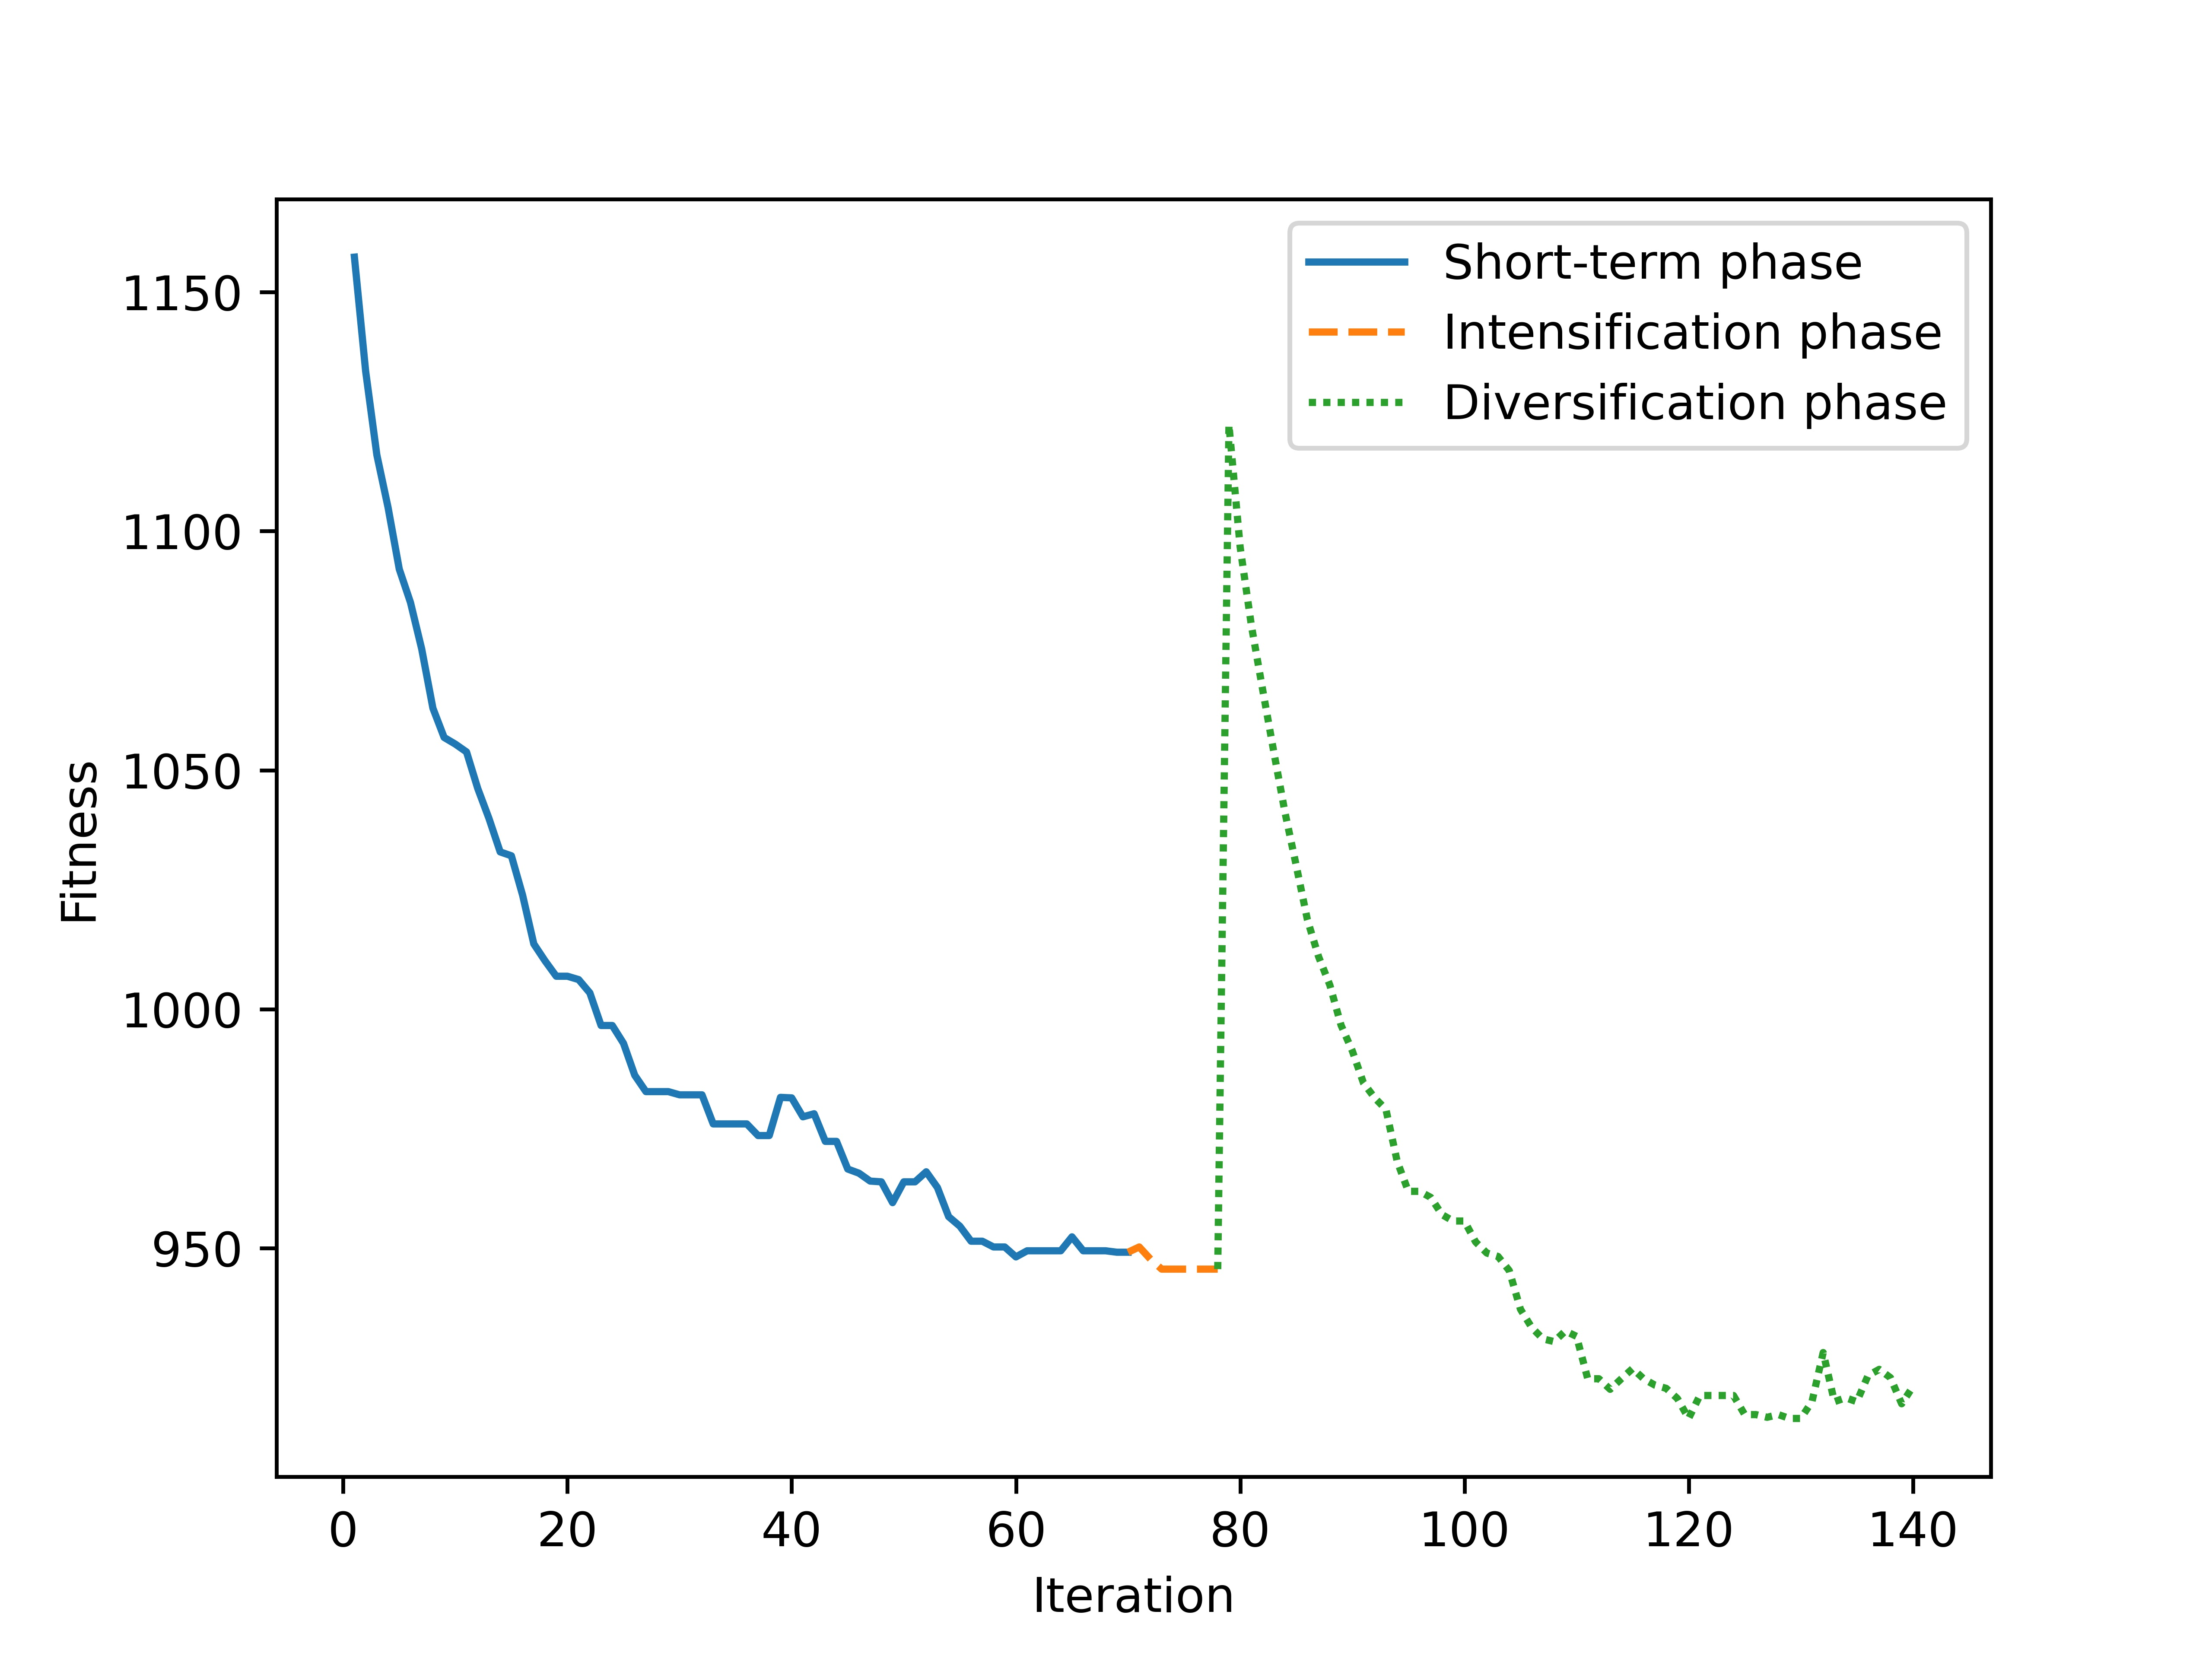
\includegraphics[width=0.95\textwidth]{images/converge_1.jpg}
        \caption{CMT07}
    \end{subfigure}
    \begin{subfigure}[b]{0.49\linewidth}
        \centering
        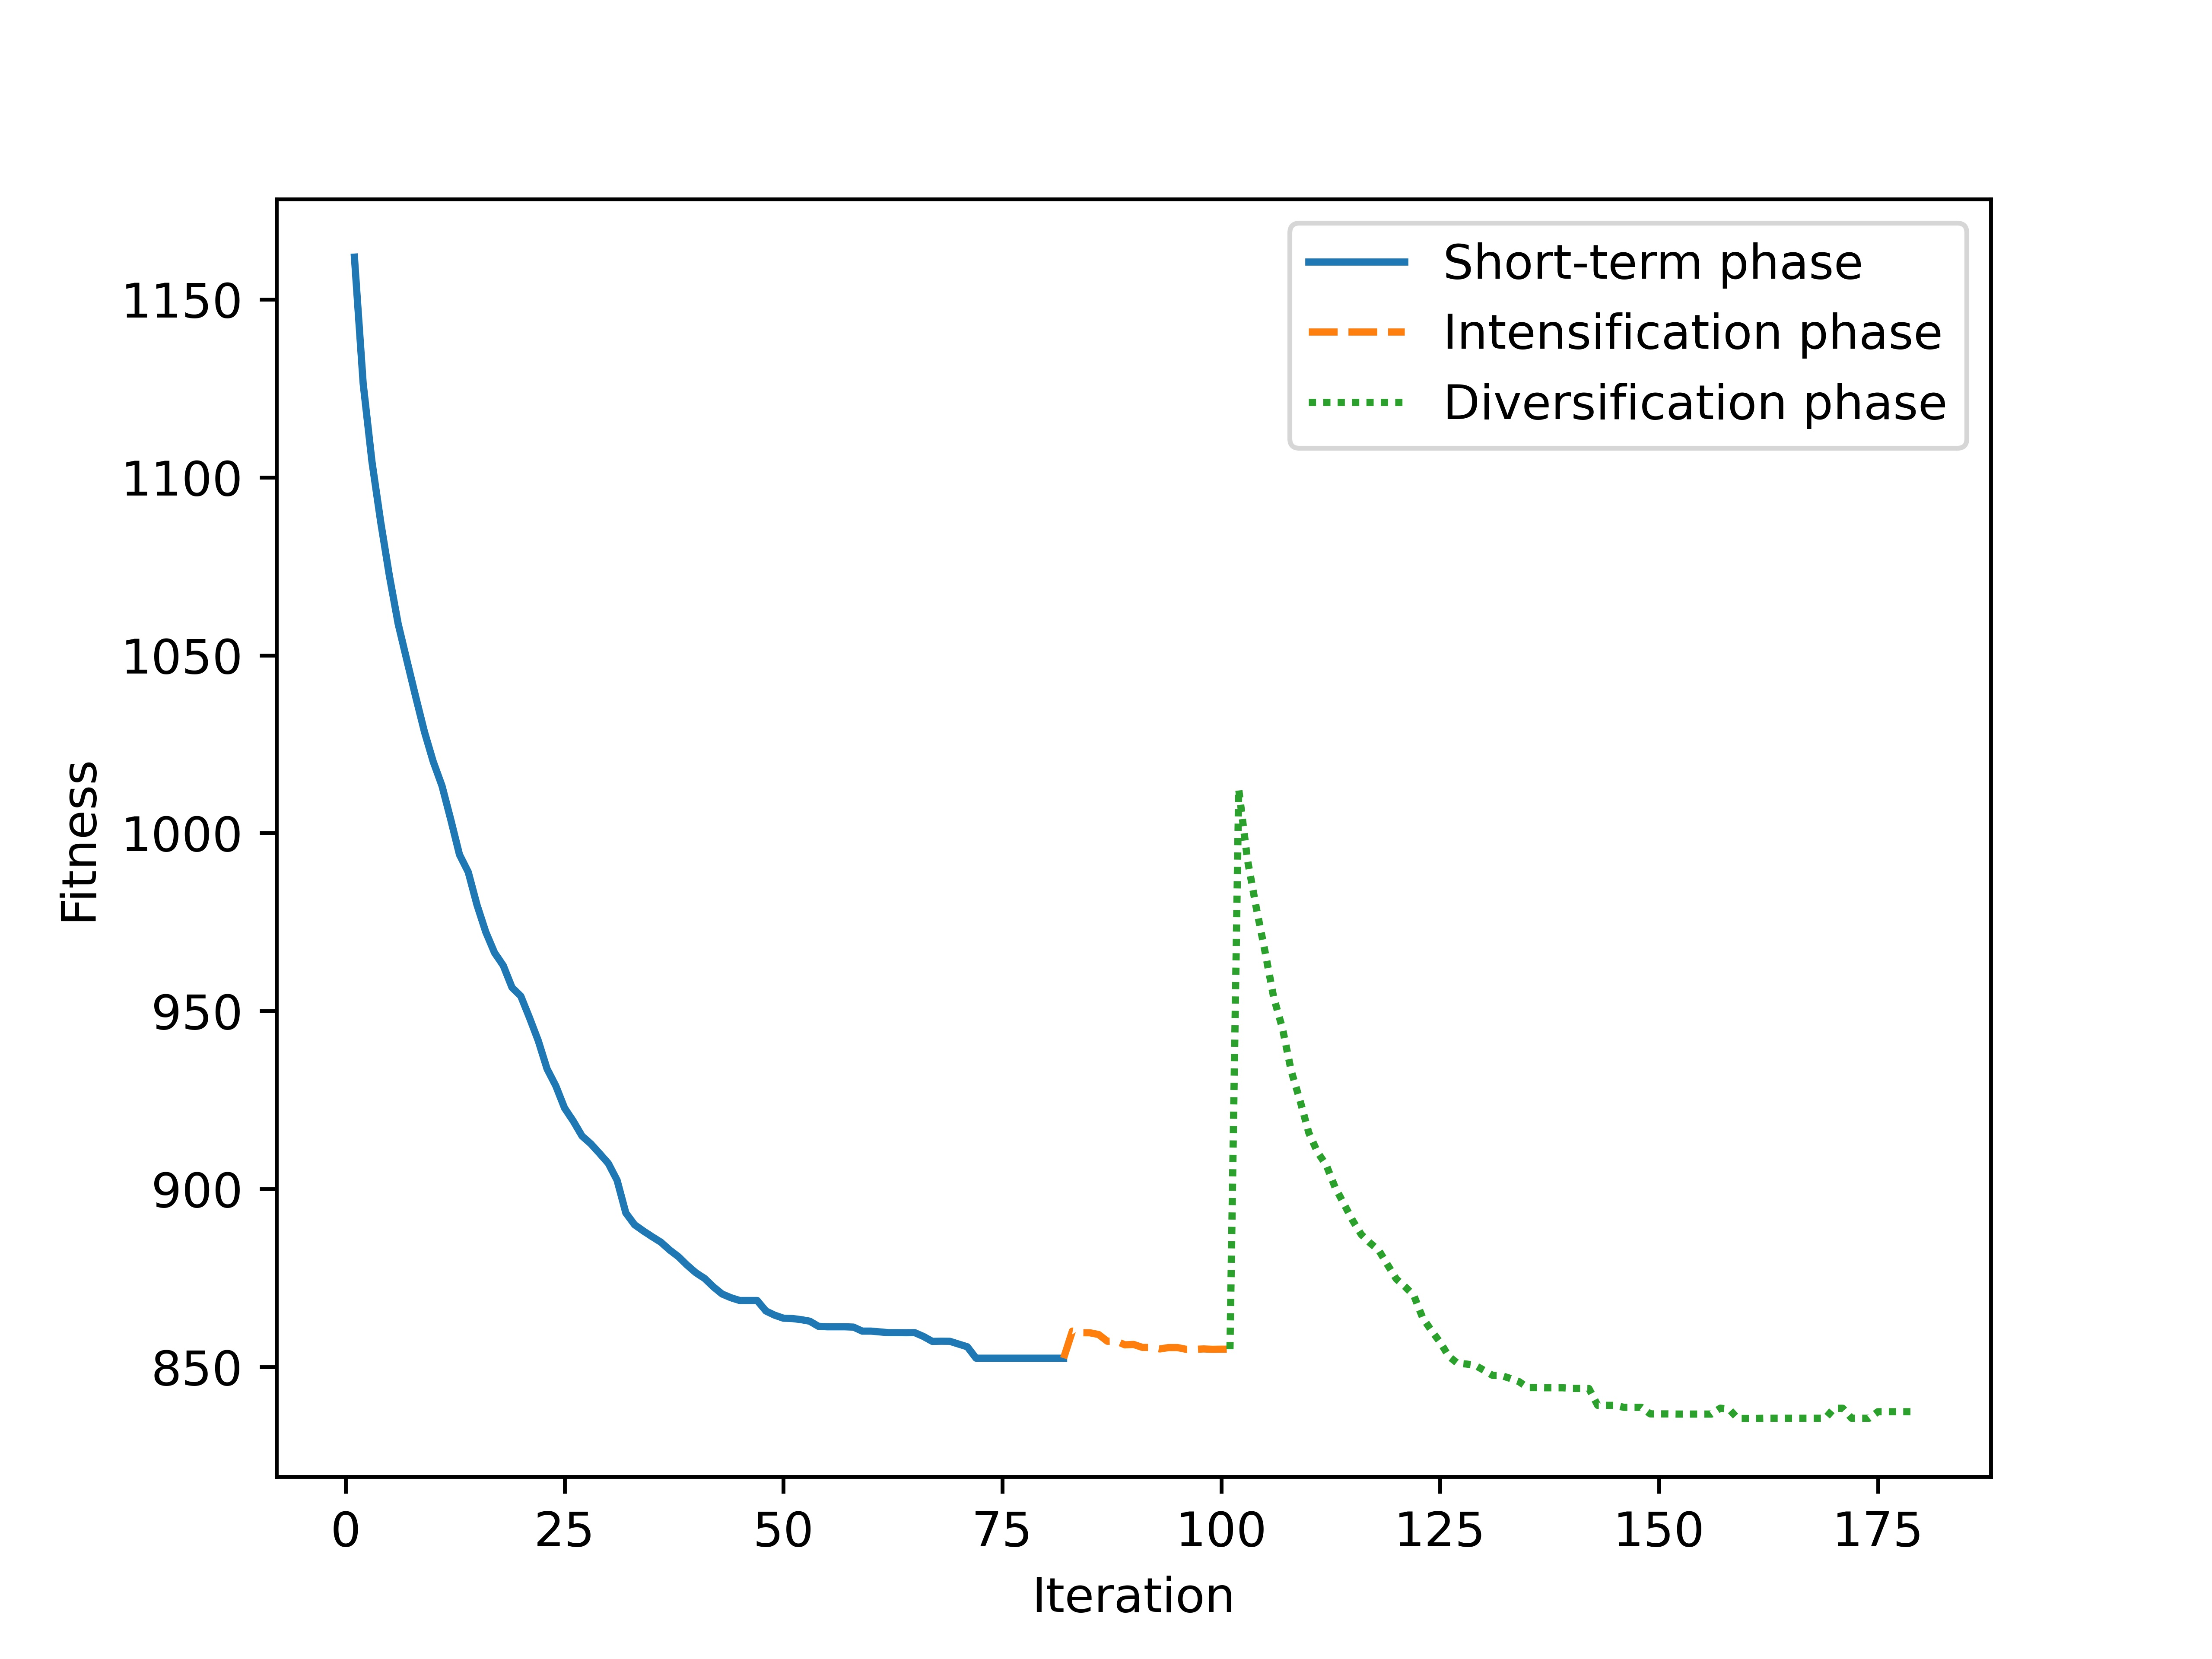
\includegraphics[width=0.95\textwidth]{images/converge_2.jpg}
        \caption{CMT12}
    \end{subfigure}
    \caption{Sample convergence charts for SimpleTabu}
\end{figure}

\begin{figure}
    \centering
    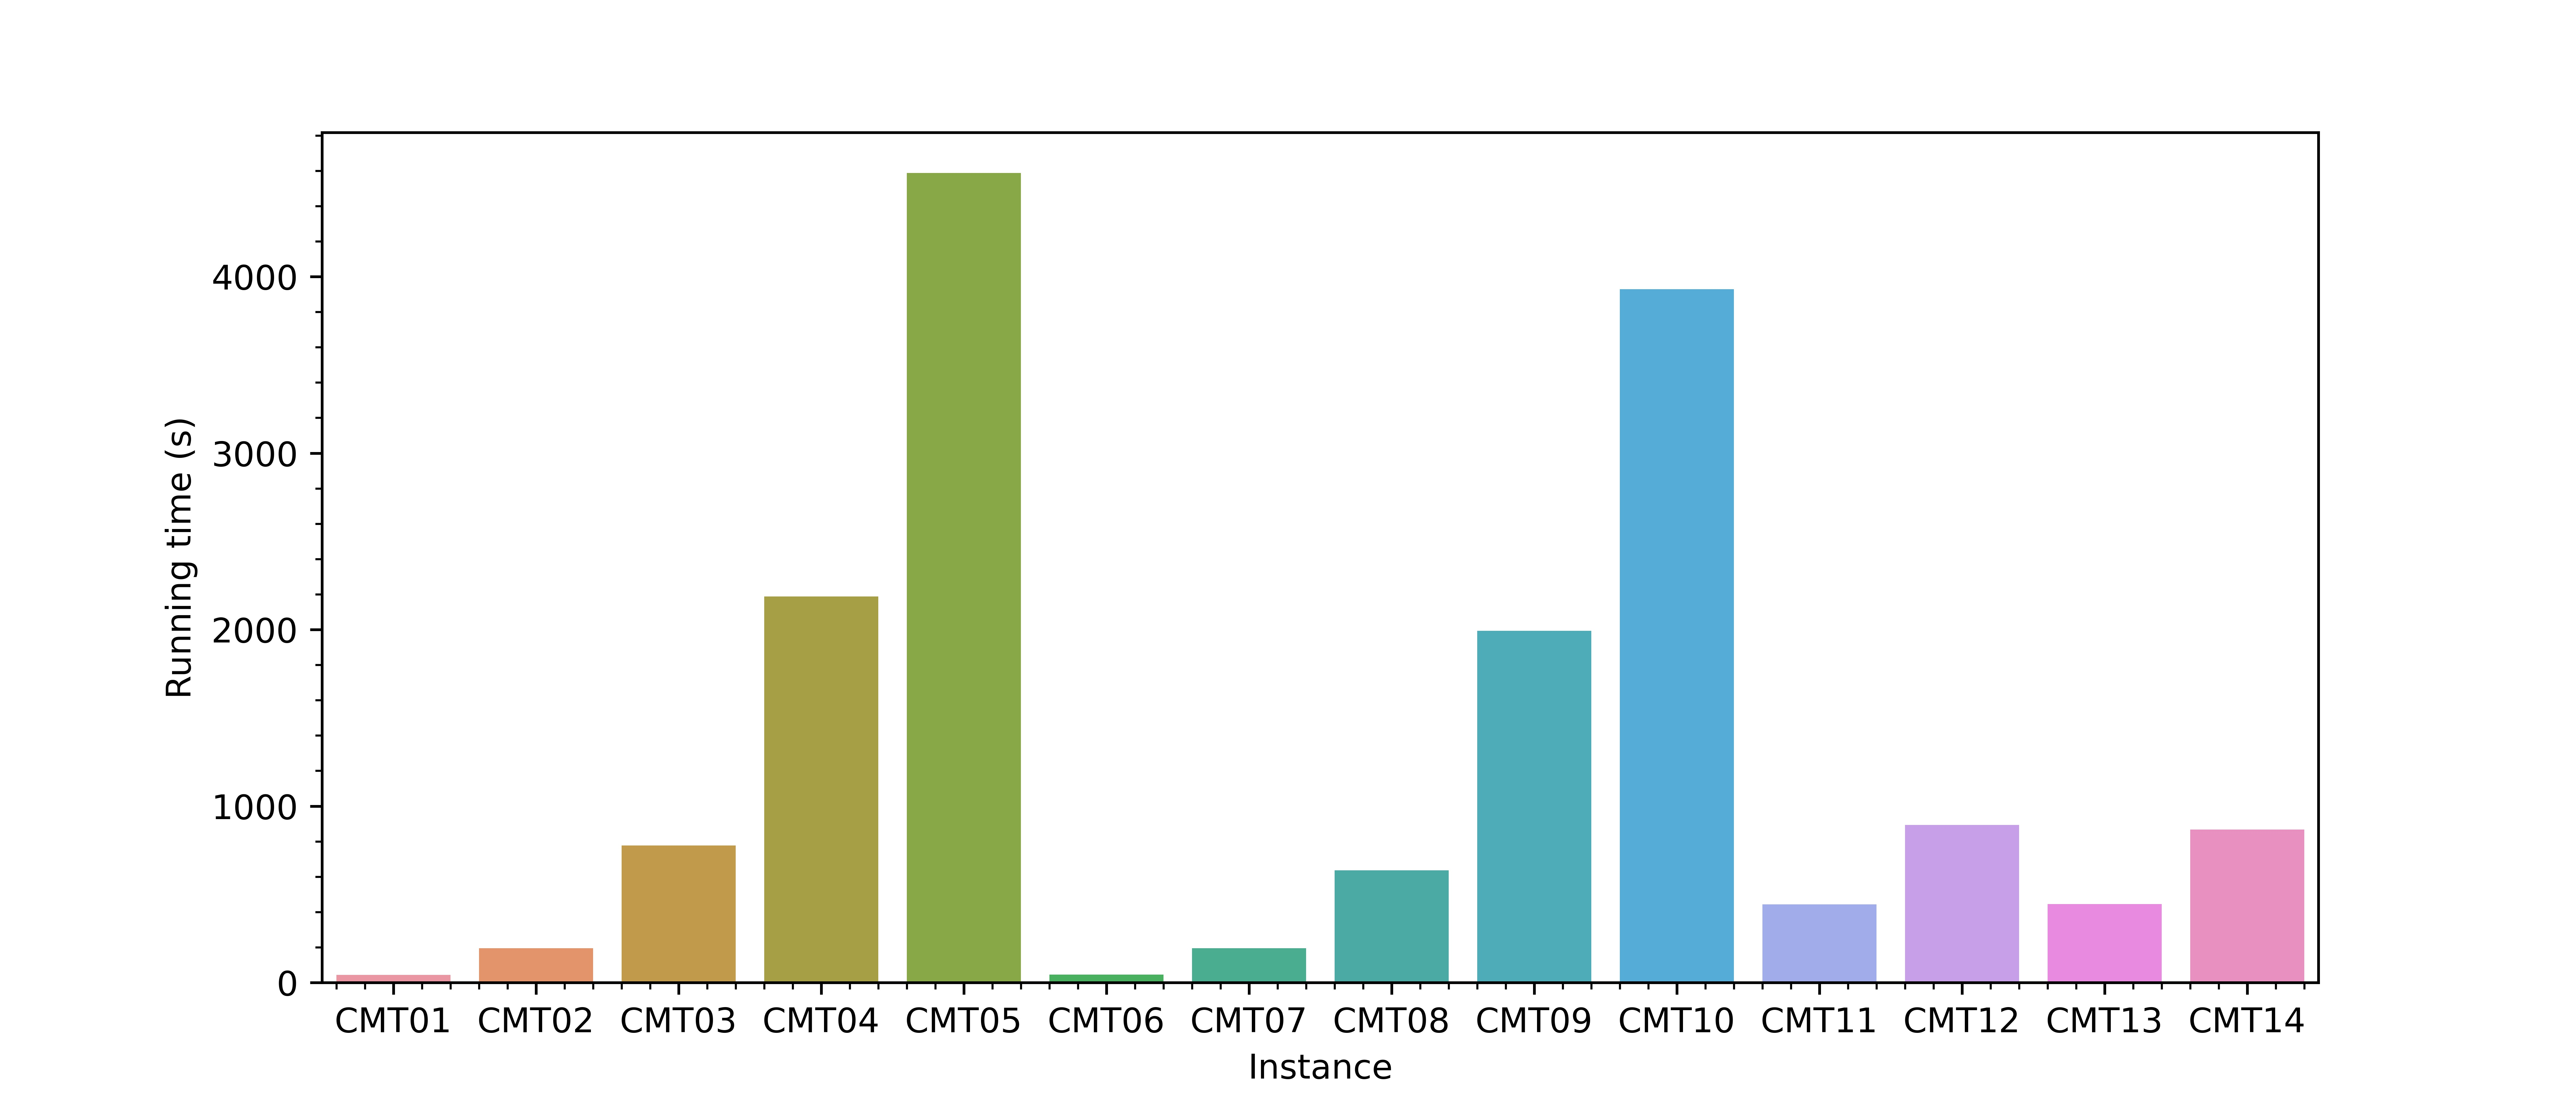
\includegraphics[width=\textwidth]{images/runtime_cmt.jpg}
    \caption{Average execution time over 5 runs for SimpleTabu on the Christofides 1979 dataset}
\end{figure}

\chapter{Conclusion}
This report has given a brief overview of Tabu search in the context of solving CVRP, a fundamental discrete optimization problem. We examined SimpleTabu, a basic implementation that, despite its simplicity, has achieved promising results on the popular CMT dataset. This goes further to show that tabu search can be a powerful search strategy for discrete problems. We also saw that the selection of neighbors can be very crucial to a search algorithm's success.

\bibliographystyle{plain}
\bibliography{report.bib}

\end{document}
